\documentclass{article}
\usepackage{kotex} % for korean support
\usepackage{color}
\usepackage{mathtools} % for pmatrix command - 행렬 표시
\usepackage{hyperref} % for hyperlink
\usepackage[margin=0.5in]{geometry} % for document margin
\usepackage{polynom} % automatic polynomial calculations(divisions, more specifically)
\usepackage{tikz}
\usepackage{siunitx} % package for angle(degree) character display
\usepackage{graphicx} % package for tikz figure caption
\usepackage{caption} % tikz figure caption\
\usepackage{graphicx} % for image files
\graphicspath{ {./images/} } % for image files

% 주의점: $로 감싸야만 사용 가능한 수식이 있고, 감싸지 않아도 사용 가능한 수식이 있으니 주의하자

\title{Highschool Geometry 고등수학 도형}
\author{박성렬}

\begin{document}
\maketitle
\captionsetup[figure]{labelfont={bf},labelformat={default},labelsep=period,name={Fig.}}
\section{용어}
\subsection{isosceles triangle}
이등변 삼각형 - 두 변의 길이가 같은 삼각형
\subsection{equilateral triangle}
정삼각형 - 세 변의 길이가 모두 같은 삼각형

\section{기본개념}
\subsection{회전 Rotation}
도형의 회전을 알아보고자 할 때에는, 도형의 회전이 일어났다고 예상되는 지점에 점을 먼저 찍어야 한다. 회전이 이루어난 점을 기준으로 기존의 점 A와 새로운 점 'A를 찍어서 연결하면 회전이 일어난 각이 나온다.\\
$$
\begin{tikzpicture}

\draw (1,3) -- (-1,1.5) -- (2,1.5);
\node at (1,3.5) {\\A};
\node at (-1,1.5) {};
\node at (2.5,1.5) {\\`A};
\draw (-0.234,2.1428) arc (40.0022:0:1);
\end{tikzpicture}
$$
\subsubsection{회전의 수학적 정의}
회전을 수로 나타날 때 직관과는 반대로 양수가 시계 반대방향이고 음수가 시계 방향이므로 유의하자.\\
시계 반대 방향으로 90도 회전($\ang{+90}$)은 다음과 같이 나타낼 수 있다:  $(x, y) ->(-y,x)$ 따라서 어떤 각이 주어지면 그것을 90도로 나눌 수 있을 경우 90도 회전을 필요한 만큼 반복하면 된다.
한편 시계 방향으로 90도 회전($\ang{-90}$)할 때에는 또 다르므로 유의하자. $(x, y) -> (y,-x)$\\
$$
\begin{tabular} {| l | l |}
\hline
이동한 각도 & 원래 형태 $(x,y)$ 에서 변한 형태\\
\hline
\ang{+90} & $(-y,x)$\\
\hline
\ang{-90} & $(y,-x)$\\
\hline
\ang{+180} & $(-x,-y)$\\
\hline
\end{tabular}
$$
도표를 참조하면 좀더 쉽다. 헷갈릴 때 이 도표를 머릿속에 그려보자.
$$
  \begin{tikzpicture}
	\node (v1) at (-6,0.5) {};
	\node (v2) at (0,0.5) {};
	\node (v3) at (-3,2.5) {};
	\node (v4) at (-3,-2) {};
	\draw  (v1) edge (v2);
	\draw  (v3) edge (v4);
	\node at (-4.5,1.5) {$-y,x$(90 deg)};
	\node at (-1.5,1.5) {$x,y$};
	\node at (-4.5,-0.5) {$-x,-y$(180 deg)};
	\node at (-1.5,-0.5) {$y,-x$(-90 deg)};
  \end{tikzpicture}
$$
\subsection{반사 Reflection}
도형의 반사는 어렵게 생각할 것 없이 기준선이 있고, 그 기준선과의 길이만 비교하면 된다. 가로축은 유지하되 세로축만 반전시키면 된다. 만약 기준선이 기울어진 상태에서도 마찬가지다.
$$
\begin{tikzpicture}

\node (v1) at (-2,-2) {};
\node (v2) at (1.5,1.5) {};
\node (v5) at (1,-1) {};
\node (v4) at (0,0) {};
\node (v3) at (-1,1) {};
\draw  (v3) edge (v4);
\draw  (v5) edge (v4);
\node at (1.5,-2) {distance = 2 block};
\draw [dash pattern=on 2pt off 3pt on 4pt off 4pt] (v2) edge (v1);
\node at (-2,2) {reflected distance = 2 block};
\end{tikzpicture}
$$
\subsection{도형의 축소와 확대 Dilation}
도형의 축소와 확대는 항상 기준점이 필요하다. 확대/축소 이후의 도형을 구하려면 기준점에서 도형의 각 꼭지점의 가로/세로 거리를 확대 또는 축소하는 비율로 곱하면 된다.
\subsection{도형의 일치 Congruence}
도형의 일치는 SSS를 외우면 된다. 삼각형의 경우 세 면(Side, Side, Side)이 일치하면 크기와 각이 모두 같은 도형이다. 그러나 ASS(Angle, Side, Side)처럼 각이 하나만 같은 도형이나 AAA처럼 각만 같은 도형은 반드시 같은 도형이 된다고 보기 어렵다.(이름이 웃겨서 외우긴 쉬울 것 같다) 왜냐면 면이 더 길수도 있기 때문이다. ASS는 마주보는 두 면이 나머지 한 면보다 모두 길 때에만 일치되고 나머지는 일치하지 않는다. \\반면 SAS, ASA, AAS는 SSS와 마찬가지로 모두 일치하는데 그건 직접 그려보는 편이 더 빠르다.\\
{\color{red} 유의점}:어떤 도형끼리 일치한다는 것은 두 도형의 비율이 일치한다는 것임에 유의하자.\\
\url{https://www.khanacademy.org/math/geometry/hs-geo-congruence/modal/a/triangle-congruence-review}
$$
\begin{tabular} {| l | l |}
\hline
일치 형태 & 일치 여부\\
\hline
AAA & X\\
\hline
SSS & O\\
\hline
SAS & O\\
\hline
ASA & O\\
\hline
AAS & O\\
\hline
SSA & 특수한 경우에만 O\\
\hline
\end{tabular}
$$
\subsection{angle bisector theorem 삼각형의 각도 양분 이론}
$$
\begin{tikzpicture}

\node (v1) at (-0.5,3) {};
\node (v2) at (-3,0) {};
\node (v3) at (1.5,0) {};
\draw (v1) -- (v2) -- (v3) -- (v1);
\node (v4) at (-0.5,0) {};
\draw  (v1) edge (v4);
\node at (-0.5,4) {A};
\node at (-4,-1) {B};
\node at (2.5,-1) {C};
\node at (-0.5,-1) {D};
\draw (-1.7656,1.48) arc (-129.7818:-56.4686:1.9779);
\node (v5) at (-1,1.5) {};
\node (v6) at (-1.5,1) {};
\node (v7) at (0,1.5) {};
\node (v8) at (0.5,1) {};
\draw  (v5) edge (v6);
\draw  (v7) edge (v8);
\end{tikzpicture}
$$
위와 같은 삼각형 $\Delta ABC$에 대해서 각도 $\widehat{ABC}$를 정확히 절반 양분하는 선 $\overline{AD}$가 있다고 할 때, $\frac{\overline{BD}}{\overline{AB}} = \frac{\overline{CD}}{\overline{AC}}$이다. 즉 $\overline{AD}$가 아닌 나머지 면들의 길이에 대한 비율이 양측이 동일하다는것!\\
{\color{red}주의} 여기서 내가 자주 헷갈렸거나 잊어버린 용어:
\begin{itemize}
  \item{perpendicular - 직각}
  \item{round - \underline{반}올림 - 반이라는 개념보다 다른 수에 가까운 수로 올림이라고 기억하면 편함. 5는 0에 가깝고, 6은 10에 가깝다!}
\end{itemize}
\subsection{special right triangles 유용한 정삼각형들}
\subsubsection{\ang{45}-\ang{45}-\ang{90} 삼각형}
제일 평범한 유형의 정삼각형. 빗변을 제외한 양 변의 길이가 같으므로 빗변만 알아도 양 변의 길이를 알 수 있다. 빗변의 길이로 양변의 길이 구하기, 또는 양변의 길이로 빗변을 구하는 식의 유도 과정은 아래와 같다.\\
*c는 빗변(hypoteneuse)이고, a와 b가 나머지 변이다. 여기서 a와 b는 길이가 동일하므로 바꿔 읽어도 된다.
$$a^{2}+b^{2}=c^{2}$$
$$b^{2}+b^{2}=c^{2}$$
$$2b^{2}=c^{2}$$
$$b^{2}=\frac{c^{2}}{2}$$
$$b=\sqrt{\frac{c^{2}}{2}}=\frac{c}{\sqrt{2}}$$
\subsubsection{\ang{30}-\ang{60}-\ang{90} 삼각형}
이것도 마찬가지로 한 변의 길이만 알아도 나머지를 추적할 수 있다. \ang{60}-\ang{90}의 각도를 가진 변은 빗변h의 $\frac{1}{2}$이다.
$$
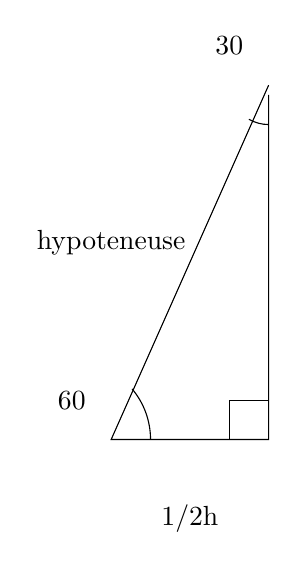
\begin{tikzpicture}

\draw (2,3) node (v1) {} -- (0,-1.5) -- (2,-1.5) -- (v1);
\draw (0.5,-1.5) arc (0:40:1);


\draw (2,2.5) arc (-89.999:-120:0.5);
\draw  (2,-1) rectangle (1.5,-1.5);
\node at (-0.5,-1) {60};
\node at (1.5,3.5) {30};
\node at (0,1) {hypoteneuse};
\node at (1,-2.5) {1/2h};
\end{tikzpicture}
$$
이 $h\frac{1}{2}$변을 기준으로 알려지지 않은 변 x의 길이를 구하는 수식은 아래와 같이 유도한다.
$${\frac{1}{2}h}^{2}+x^{2}=h^{2}$$
$$\frac{h^{2}}{4}+x^{2}=h^{2}$$
$$x^{2}=h^{2}(1-\frac{1}{4})$$
$$x^{2}={\frac{3}{4}h}^{2}$$
$$x={\frac{\sqrt{3}}{2}}{\cdot}h$$
\subsection{basics of trigonometry - trigonometric ratios 삼각법 기본 - 삼각률}
삼각법은 정삼각형을 기준으로 사용하며, 하나의 각을 대상으로 한다.
$$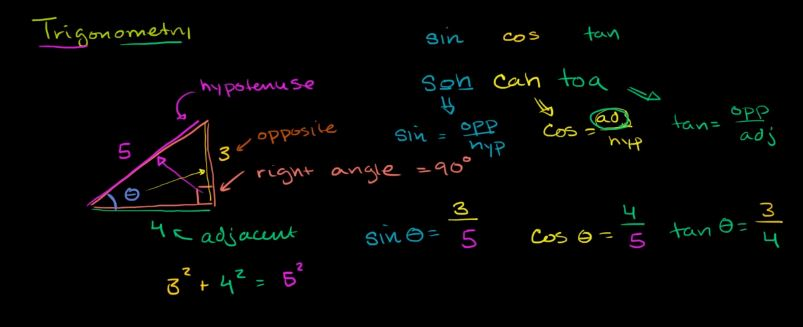
\includegraphics[scale=0.8]{trigonometry.jpg}$$
$\theta$를 기준 각으로 봤을 때, $\sin \cos \tan$은 해당 각의 상대적 위치를 가지고 다른 변 길이들의 비율을 알려준다. 비율의 내용을 빨리 외우기 위해 soh, cah, toa로 외운다. 이는 아래의 내용을 나타낸다\\
$${\sin\theta}\textsf{(S.O.H)}=\frac{\textsf{Opposite (side)of $\theta$}}{\textsf{Hypoteneuse of $\theta$}}$$
$${\cos\theta}\textsf{(C.A.H)}=\frac{\textsf{Adjecent of $\theta$}}{\textsf{Hypoteneuse of $\theta$}}$$
$${\tan\theta}\textsf{(T.O.A)}=\frac{\textsf{Opposite of $\theta$}}{\textsf{Adjecent of $\theta$}}$$
위의 그림으로 예를 들자면 $\sin$은 $\theta$로부터 반대편의 변 길이인 3을 빗변의 길이 5로 나눈 $\frac{3}{5}$가 된다. 각을 읽는 방법이 헷갈리면 다음 페이지를 참조하자\\
\url{https://www.khanacademy.org/math/geometry/hs-geo-trig/modal/a/opposite-adjacent-hypotenuse}\\
삼각법을 이용할 때에는 먼저 대상 각을 결정한다. 이때 대상 각은 직각이 될 수 없다. 직각은 이웃한 변이 두 가지이고, 빗변이 곧 반대편의 변이 되기 때문에, 때문에 정의가 애매해진다. 따라서 위의 $\theta$를 기준으로 적용하고자 한다면, $\sin{\theta}=\frac{3}{5}$가 된다. 여기서 $\theta$의 정확한 각도 값만 알 수 있으면 하나의 변만 주어져도 길이를 알 수 있다. 예를 들어 반대편 변인 3의 길이를 모른다고 할 경우,
$$\sin{\theta}=\frac{x}{5}$$
$$\sin{\theta}{\cdot}5=x$$
여기서 계산기에 $\sin{\theta}$를 입력하고 곱하기 5를 하면 x의 변이 나오는 것이다! \\
즉, 삼각법을 알고 있으면 정삼각형에서 직각을 제외한 다른 두 각 중 하나의 각과 하나의 변 길이만 알아도 나머지 두 변의 길이를 모두 알 수 있다.
\subsection{inverse trigonomy functions 역 삼각법}
삼각법을 역으로 적용하여 두 변의 길이만 아는 상태에서 각도를 알아내고자 한다면, 역 삼각법을 적용한다. 역 삼각법은 $\sin^{-1}$과 같은 형식으로 $^{-1}$로 표기하며, 일반적인 승수 표현과 달리 $\frac{1}{x}$가 아니다. 따라서 프로그래밍에서는 이를 $\arccos \arcsin \arctan$

\end{document}